\documentclass{../../tex_template/asaproc}
\usepackage{graphicx} % \includegraphics
\usepackage{float}    % To keep figures in right place. 
                      % Usage: \being{figure}[H] \includegraphics{tmp.pdf} \end{figure}
\usepackage{subfig}   % \subfloat
\usepackage{amsmath}  % bmatrix, pmatrix, etc
\usepackage{bm}
\newcommand{\p}[1]{\left(#1\right)}
\newcommand{\bk}[1]{\left[#1\right]}
\newcommand{\bc}[1]{ \left\{#1\right\} }
\newcommand{\abs}[1]{ \left|#1\right| }
\newcommand{\norm}[1]{ \left|\left|#1\right|\right| }
\newcommand{\E}{ \text{E} }
\newcommand{\N}{ \mathcal N }
\newcommand{\ds}{ \displaystyle }

%\usepackage{times}
%If you have times installed on your system, please
%uncomment the line above

%For figures and tables to stretch across two columns
%use \begin{figure*} \end{figure*} and
%\begin{table*}\end{table*}
% please place figures & tables as close as possible
% to text references

\newcommand{\be}{\begin{equation}}
\newcommand{\ee}{\end{equation}}
\newcommand{\y}{\bm y}
\newcommand{\X}{\bm X}
\newcommand{\Xb}{\bm {X\beta}}

\title{FYE--- Ozone}

%input all authors' names
\author{
  Arthur Lui$^1$\\
  University California -- Santa Cruz$^1$\\
}

%input affiliations
%{USDA Forest Service Forest Products Laboratory}

\begin{document}
\maketitle
\begin{abstract}
Exposure to high ozone levels is known to be associated with the development
of respiratory and other illnesses. Hence, modeling ozone levels is of interest
to climatoligists and medical professionals. The effects on ozone levels by
temperature, wind speed and radiation are explored using a g-prior in this 
paper. The results of the analysis show that all three of these variables are
important in predicting ozone concentrations. In addition, a model with
radiation as a covariate substantially the Bayes factor beyond the model
that does not include radiation.

\begin{keywords}
Bayesian Regression, ozone, temperature, wind speed, radiation, g-priors
\end{keywords}
\end{abstract}

\section{Introduction}
Exposure to high ozone levels is known to be associated with the development of
respiratory and other illnesses. Ozone levels are typically measured in terms
of concentration (parts per billion or simply ppb). Ozone levels of 70ppb are
considered high or dangerous. Hence, modeling ozone levels is an area of 
concern to medical professionals, scientists, as well as governments. In this
study, the effects of radiation (0 for low, 1 for moderate to high levels), 
temperature (F$^\circ$), and wind speed (mph) are explored using a Bayesian
regression model which makes use of Zellner's g-prior as the prior for covariates
in the model. Of particular interest in this paper is whether including the 
radiation variable in the model improves the model that does not include it.
Using a g-prior-based regression model, computing the Bayes factors for competing
models becomes simple.\\

This remainder of this paper is divided into 4 parts. The first part is an 
exploratory analysis of the data. The next part outlines the methods used in
the analysis and model fitting. This section will include a brief overview
of Zellner's g-prior. The next section contains the results of the analysis.
The final section contains concluding remarks and items for future studies.

\section{Exploratory Analysis}
The data provided consists of 111 rows (observations) and 4 columns -- the
first column being ozone concentration, and the remaining columns being the
values corresponding to each of the aforementioned variables. The data is
plotted as a scatter plot matrix as shown in Figure \ref{fig:pairs} Along the
diagonal are the univariate histograms for each of the variables. Displayed in the
lower traingle are the correlations between each pairs of covariates. (The 
value .464 corresponds to the correlation between ozone and radiation, etc.)
The upper triangle displays the scatter plot for each pair of variables.\\

\begin{figure}[H]
  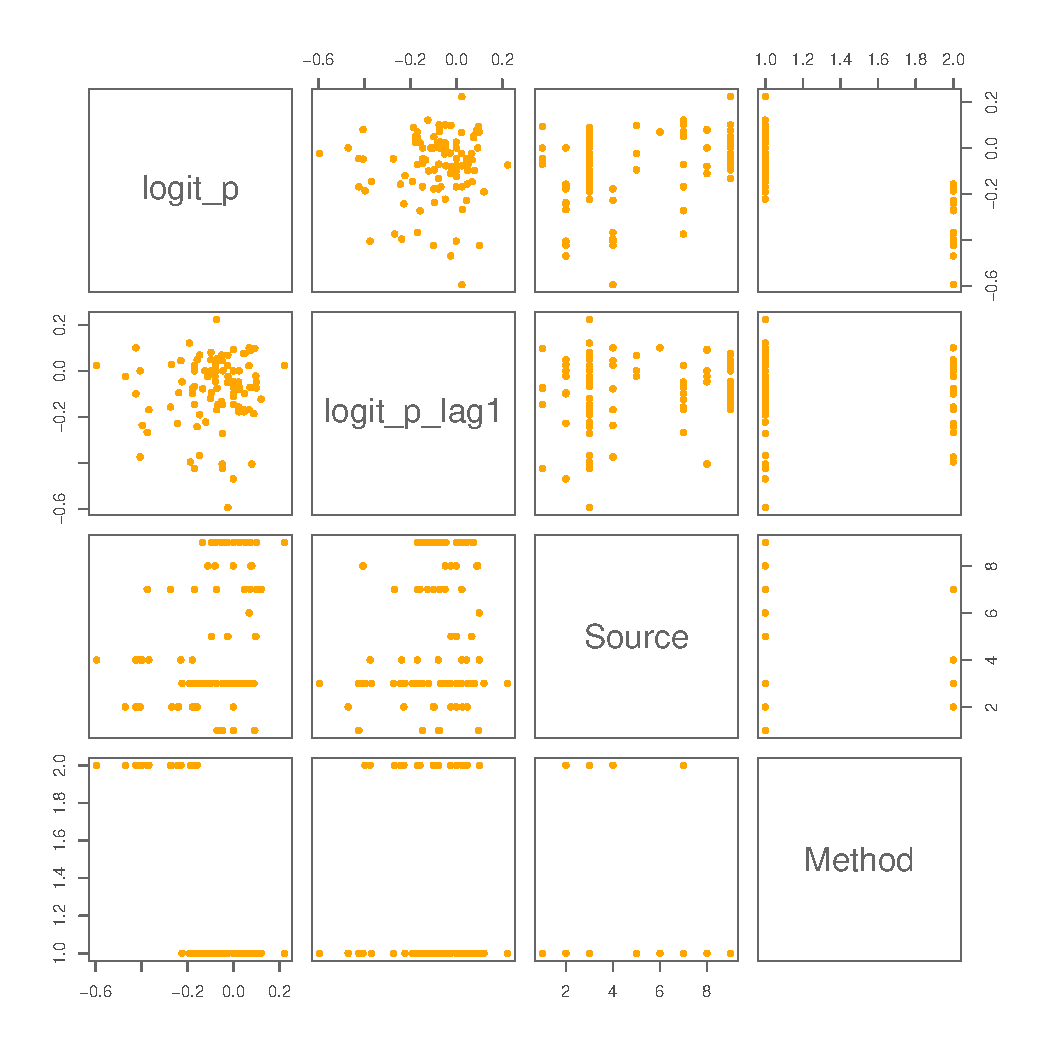
\includegraphics[scale=.5]{figs/pairs.pdf}
  \caption{\small Scatter plot matrix of ... }
  \label{fig:pairs}
\end{figure}

A first observation is that ozone concentrations appear non-linearly related to
all of the variables. To exploit the simplicity of linear models, a log
transform is imposed on ozone concentrations. The resulting data is shown in
Figure \ref{fig:logpairs}. After the transformation, the data indeed exhibit a
linear trend between ozone and the other variables. Another item to note is
that the variables are at most moderately linearly correlated with one another.
(Ozone and temperature have the largest correlation of .75.) This is a
desireable property in regression models as high correlation between covariates
often leads to inflated variances of the estimated coefficients. Also note that
the range for each variable is very different. Log-ozone ranges from 0 to 5.12,
radiation is a binary variable, temperatures range from 57 to 97 F$\circ$, and
wind speeds range from 2.3 to 20.7 mph. Taking this variability in ranges into
consideration, it may be appropriate to center and scale the variables while
doing a regression analysis. For simplicity, this step is omitted.

\begin{figure}[H]
  \includegraphics[scale=.5]{figs/log_ozone_pairs.pdf}
  \caption{\small Scatter plot matrix of ... }
  \label{fig:logpairs}
\end{figure}

Given this preliminary analysis, a good candidate linear model is that with
response variable $\y$ being the log ozone concentration, and covariates being
radiation level, temperature, and wind speed. This is a good candidate model
because log-ozone concentration is linear with the covariates and the 
covariates are not strongly correlated.

\section{Methods}
The linear model used in this analysis is a Bayesian linear regression model
using Zellner's g-prior for the covariates. As mentioned, this model is both
simple to fit, and provides easy diagnostics for model comparison using 
Bayes factors.\\

A regression model that uses g-priors is typically specified as follows:
\[
  \begin{array}{rclcl}
    \y &|& \X,\bm\beta,\phi &\sim& \mathcal{N}_n\p{\Xb,\frac{1}{\phi}\bm I_n} \\
       && p(\bm\beta,\phi) &\propto& \frac{1}{\phi} \mathcal{N}_k (\bm 0, \frac{g}{\phi} (\X^T\X)^{-1})\\
  \end{array}
\]
where $\X$ is the matrix of covariates with a column of ones in prepended, $\y$
is the response variable, $\phi$ is the model precision, $n$ is the number of
observations, $k$ is the number of covariates, and $g$ is a constant to be
determined. There are many ways to determine a good choice for $g$ but should
typically be chosen to be large. In this study $g$ is to set be $n$. 

\section{Analysis}
ANALYSIS GOES HERE!!!
\begin{figure}[H]
  \includegraphics[scale=.5]{figs/posts1.pdf}
  \caption{\small Posteriors of ... }
  \label{fig:posts1}
\end{figure}

\begin{figure}[H]
  \includegraphics[scale=.5]{figs/posts2.pdf}
  \caption{\small Posteriors of ... }
  \label{fig:posts2}
\end{figure}

\begin{figure}[H]
  \includegraphics[scale=.5]{figs/obsvsfit.pdf}
  \caption{\small Posteriors of observed vs. fitted. }
  \label{fig:obsvsfit}
\end{figure}

\begin{figure}[H]
  \includegraphics[scale=.5]{figs/rmse.pdf}
  \caption{\small Posteriors of RMSE. The model with radiation has lower RMSE.
    The probability that the RMSE in the model with radiation as a coavariate
    is lower than that of the model without radiation is 84\%.}
  \label{fig:rmse}
\end{figure}

\begin{figure}[H]
  \includegraphics[scale=.5]{figs/map.pdf}
  \caption{\small Heatmap of ...}
  \label{fig:map}
\end{figure}

\begin{figure}[H]
  \includegraphics[scale=.5]{figs/marginal.pdf}
  \caption{\small Marginal Posterior}
  \label{fig:marginal}
\end{figure}

\section{Conclusions}
CONCLUSIONS GO HERE!!!

\begin{references}
{\footnotesize
\itemsep=3pt
\item {\em Gelman, A., Carlin, J. B., Stern, H. S., \& Rubin, D. B. (2014). Bayesian data analysis (Vol. 2). Boca Raton, FL, USA: Chapman \& Hall/CRC, 73.}
}

\end{references}
\end{document}

%\begin{figure*}
%  \centering
%  \includegraphics[scale=.55]{figs/mapDat.pdf}
%  \vspace{-7em}
%  \caption{\small Some Caption.}
%  \label{fig:mapDat}
%\end{figure*}

%\begin{figure}[H]
%  \includegraphics[scale=.5]{figs/pairsLogRate.pdf}
%  \caption{\small Hi Motor vehicle theft is not strongly correlated with any other thefts.}
%  \label{fig:logOdds}
%\end{figure}
